
Il moto di un elemento infinitesimo di fluido può essere descritto come composizione di una traslazione, di una rotazione rigida e una deformazione.
Siano $\bm{x}_1(t)$, $\bm{x}_2(t)$ le posizioni di due punti materiali e $\delta\bm{x}(t) = \bm{x}_2(t) - \bm{x}_1(t)$ il vettore che congiunge questi due punti.
La derivata temporale del vettore $\delta \bm{x}(t)$ può essere scritta come
\begin{equation}
 \frac{d \delta\bm{x}}{d t}(t) =
  \frac{d \bm{x}_2}{d t}(t) - \frac{d \bm{x}_1}{d t}(t) = 
  \bm{u}(\bm{x}_2(t),t) - \bm{u}(\bm{x}_1(t),t) \ , 
\end{equation}
avendo sfruttato la definizione di punto materiale per esprimere la sua velocità,
$d \bm{x}_i/dt$, come la velocità del continuo in quel punto, $\bm{u}(\bm{x}_i(t),t)$.
\newline \noindent
Utilizzando la definizione di $\delta \bm{x}(t)$, si può scrivere $\bm{x}_2(t) = \bm{x}_1(t) + \delta \bm{x}(t)$ ed esprimere la velocità calcolata in $\bm{x}_2(t)$ con un'espansione in serie centrata in $\bm{x}_1(t)$,
\begin{equation}
\begin{aligned}
    \bm{u}(\bm{x}_2(t),t) & = \bm{u}(\bm{x}_1(t)+\delta\bm{x}(t),t) = \\
    & = \bm{u}(\bm{x}_1(t),t) + \delta\bm{x}(t) \cdot \bm{\nabla} \bm{u}(\bm{x}_1(t),t) +
    o(|\delta\bm{x}(t)|) \ .
\end{aligned}
\end{equation}
Utilizzando la notazione tensoriale, si può quindi scrivere la derivata temporale di $\delta \bm{x}$ come
\begin{equation}\label{eqn:ddxdt:tens}
 \frac{d \delta \bm{x}}{d t}(t) = \delta \bm{x}(t) \cdot \bm{\nabla}\bm{u}(\bm{x}_1(t),t) + o(|\delta\bm{x}(t)|) \ .
\end{equation}
Utilizzando un sistema di coordinate cartesiane e la base naturale ortornormale $\{ \bm{\hat{x}}, \bm{\hat{y}}, \bm{\hat{z}} \}$, si può scrivere l'espressione (\ref{eqn:ddxdt:tens}) in componenti,
\begin{equation}
\begin{cases}
 \dfrac{d \delta x}{d t} =  x \p{u_x}{x} + y \p{u_x}{y} + z \p{u_x}{z} \\
 \dfrac{d \delta y}{d t} =  x \p{u_y}{x} + y \p{u_y}{y} + z \p{u_y}{z} \\
 \dfrac{d \delta z}{d t} =  x \p{u_z}{x} + y \p{u_z}{y} + z \p{u_z}{z} \\
\end{cases} \quad , \qquad 
 \dfrac{d \delta x_i}{d t} =  x_k \p{u_i}{x_k} 
\end{equation}


Il tensore del secondo ordine \textit{gradiente della velocità} $\bm{\nabla} \bm{u}$ può essere scritto come somma della sua parte simmetrica e della sua parte antisimmetrica, rispettivamente il \textit{tensore velocità di deformazione} $\mathbb{D}$ e \textit{tensore di spin} $\mathbb{R}$, $\bm{\nabla} \bm{u} = \mathbb{D} + \mathbb{W}$. Questi tensori possono essere scritti utilizzando la base prodotto costruita con i vettori della base cartesiana,
\begin{equation}\label{eqn:grad}
\begin{aligned}
 \bm{\nabla} \bm{u} = & \p{u_x}{x} \bm{\hat{x}}\otimes\bm{\hat{x}} + 
                        \p{u_x}{y} \bm{\hat{y}}\otimes\bm{\hat{x}} +
                        \p{u_x}{z} \bm{\hat{z}}\otimes\bm{\hat{x}} + \\
                    + & \p{u_y}{x} \bm{\hat{x}}\otimes\bm{\hat{y}} +
                        \p{u_y}{y} \bm{\hat{y}}\otimes\bm{\hat{y}} +
                        \p{u_y}{z} \bm{\hat{z}}\otimes\bm{\hat{y}} + \\
                    + & \p{u_z}{x} \bm{\hat{x}}\otimes\bm{\hat{z}} +
                        \p{u_z}{y} \bm{\hat{y}}\otimes\bm{\hat{z}} +
                        \p{u_z}{z} \bm{\hat{z}}\otimes\bm{\hat{z}}
\end{aligned} \hspace{1.0cm}
 \left\{ \bm{\nabla}\bm{u} \right\}_{ij} = \p{u_j}{x_i} \ ,
\end{equation}
\begin{equation}\label{eqn:d}
\begin{aligned}
 \mathbb{D} = & \frac{1}{2}\left[ \p{u_x}{x} +  \p{u_x}{x} \right] \bm{\hat{x}}\otimes\bm{\hat{x}} + 
                \frac{1}{2}\left[ \p{u_x}{y} +  \p{u_y}{x} \right] \bm{\hat{y}}\otimes\bm{\hat{x}} +
                \frac{1}{2}\left[ \p{u_x}{z} +  \p{u_z}{x} \right] \bm{\hat{z}}\otimes\bm{\hat{x}} + \\
            + & \frac{1}{2}\left[ \p{u_y}{x} +  \p{u_x}{y} \right] \bm{\hat{x}}\otimes\bm{\hat{y}} +
                \frac{1}{2}\left[ \p{u_y}{y} +  \p{u_y}{y} \right] \bm{\hat{y}}\otimes\bm{\hat{y}} +
                \frac{1}{2}\left[ \p{u_y}{z} +  \p{u_z}{y} \right] \bm{\hat{z}}\otimes\bm{\hat{y}} + \\
            + & \frac{1}{2}\left[ \p{u_z}{x} +  \p{u_x}{z} \right] \bm{\hat{x}}\otimes\bm{\hat{z}} +
                \frac{1}{2}\left[ \p{u_z}{y} +  \p{u_y}{z} \right] \bm{\hat{y}}\otimes\bm{\hat{z}} +
                \frac{1}{2}\left[ \p{u_z}{z} +  \p{u_z}{z} \right] \bm{\hat{z}}\otimes\bm{\hat{z}} \\
  D_{ij} & = \dfrac{1}{2}\left[ \p{u_j}{x_i} + \p{u_i}{x_j} \right] \ ,
\end{aligned}
\end{equation}
\begin{equation}\label{eqn:w}
\begin{aligned}
 \mathbb{W} = &  \hspace{2.0cm} 0 \hspace{0.5cm}                    \bm{\hat{x}}\otimes\bm{\hat{x}} + 
                \frac{1}{2}\left[ \p{u_x}{y} -  \p{u_y}{x} \right]  \bm{\hat{y}}\otimes\bm{\hat{x}} +
                \frac{1}{2}\left[ \p{u_x}{z} -  \p{u_z}{x} \right]  \bm{\hat{z}}\otimes\bm{\hat{x}} + \\
            + & \frac{1}{2}\left[ \p{u_y}{x} -  \p{u_x}{y} \right]  \bm{\hat{x}}\otimes\bm{\hat{y}} +
                 \hspace{2.0cm} 0 \hspace{0.5cm}                    \bm{\hat{y}}\otimes\bm{\hat{y}} +
                \frac{1}{2}\left[ \p{u_y}{z} -  \p{u_z}{y} \right]  \bm{\hat{z}}\otimes\bm{\hat{y}} + \\
            + & \frac{1}{2}\left[ \p{u_z}{x} -  \p{u_x}{z} \right]  \bm{\hat{x}}\otimes\bm{\hat{z}} +
                \frac{1}{2}\left[ \p{u_z}{y} -  \p{u_y}{z} \right]  \bm{\hat{y}}\otimes\bm{\hat{z}} +
                 \hspace{2.0cm} 0 \hspace{0.5cm}                    \bm{\hat{z}}\otimes\bm{\hat{z}} \\
  W_{ij} & = \dfrac{1}{2}\left[ \p{u_j}{x_i} - \p{u_i}{x_j} \right] \ .
\end{aligned}
\end{equation}
Osservando le componenti di $\mathbb{W}$, si possono riconoscere le componenti del campo \textit{vorticità} $\bm{\omega}$, definito come il rotore del campo di velocità, $\bm{\omega} = \bm{\nabla} \times \bm{u}$ e quindi scrivere,
\begin{equation}\label{eqn:w}
\begin{aligned}
 \mathbb{W} = & \ 0 \quad               \bm{\hat{x}}\otimes\bm{\hat{x}}   
              - \frac{1}{2} \omega_z \, \bm{\hat{y}}\otimes\bm{\hat{x}} +
                \frac{1}{2} \omega_y \, \bm{\hat{z}}\otimes\bm{\hat{x}} + \\
              & \frac{1}{2} \omega_z \, \bm{\hat{x}}\otimes\bm{\hat{y}} +
                \ 0 \quad               \bm{\hat{y}}\otimes\bm{\hat{y}}  
              - \frac{1}{2} \omega_x \, \bm{\hat{z}}\otimes\bm{\hat{y}} + \\
            - & \frac{1}{2} \omega_y \, \bm{\hat{x}}\otimes\bm{\hat{z}} +
                \frac{1}{2} \omega_x \, \bm{\hat{y}}\otimes\bm{\hat{z}} +
                \ 0 \quad               \bm{\hat{z}}\otimes\bm{\hat{z}} \\
\end{aligned}
\end{equation}

Ai tensori $\mathbb{D}$ e $\mathbb{W}$ si possono associare rispettivamente di deformazione e rotazione nell'evoluzione di $\delta \bm{x}(t)$,
\begin{equation}\label{eqn:evo:1}
    \frac{d \delta \bm{x}}{d t}(t) = \delta \bm{x}(t) \cdot \mathbb{D}(\bm{x}_1(t),t) +
                                     \delta \bm{x}(t) \cdot \mathbb{W}(\bm{x}_1(t),t) + o(|\delta\bm{x}(t)|) \ .
\end{equation}
Sfruttando la natura antisimmetrica del tensore di spin $\mathbb{W}$, si può riscrivere il contributo di rotazione al movimento in una forma che dovrebbe essere più familiare, corrispondente all'atto di moto rigido, visto in meccanica razionale. Aiutandosi con l'espressione del tensore $\mathbb{W}$ si può svolgere l'operazione $\delta\bm{x} \cdot \mathbb{W}$,
\begin{equation}
\begin{aligned}
 \delta\bm{x} \cdot \mathbb{W} & = \frac{1}{2}\left[ - \delta y \omega_z + \delta z \omega_y \right] \bm{\hat{x}} +
                                   \frac{1}{2}\left[ - \delta z \omega_x + \delta x \omega_z \right] \bm{\hat{y}} +
                                   \frac{1}{2}\left[ - \delta x \omega_y + \delta y \omega_x \right] \bm{\hat{z}} = \\
  & = \frac{1}{2} \bm{\omega} \times \delta \bm{x} \ ,
\end{aligned}
\end{equation}
avendo riconosciuto l'espressione del prodotto vettoriale tra $\bm{\omega}$ e $\delta \bm{x}$. L'equazione (\ref{eqn:evo:1}) può quindi essere riscritta,
\begin{equation}
    \frac{d \delta \bm{x}}{d t}(t) = \delta \bm{x}(t) \cdot \mathbb{D}(\bm{x}_1(t),t) + 
    \frac{1}{2} \bm{\omega}(\bm{x}_1(t),t) \times \delta \bm{x}(t) + o(|\delta\bm{x}(t)|) \ ,
\end{equation}
in modo tale da mettere in evidenza i due termini che determinano l'evoluzione del vettore elementare $\delta \bm{x}$:
\begin{itemize}
 \item il termine di rotazione ``media'', $\frac{1}{2} = \bm{\omega} \times \delta \bm{x}$; ricordando la legge dell'atto di moto rigido studiata in meccanica razionale,\footnote{
  Dati due punti $\bm{r}_1$, $\bm{r}_2$ appartenenti a un corpo rigido, vale la relazione
  % \begin{equation}
  %   \frac{d\bm{r}_2}{dt} - \frac{d\bm{r}_1}{dt} = \bm{\Omega} \times \left( \bm{r}_2 - \bm{r}_1 \right) \ ,
  % \end{equation}
  dove $\bm{\Omega}$ è il vettore velocità angolare del corpo rigido.
 }
 si può riconoscere il legame tra vorticità $\bm{\omega}$ e velocità angolare di una particella materiale: la vorticità $\bm{\omega}(\bm{x},t)$ risulta essere il doppio della velocità angolare della particella materiale che passa per il punto $\bm{x}$ all'istante temporale $t$.
 \item il termine di deformazione, $\mathbb{D} \cdot \delta \bm{x}$.\footnote{
 Poiché $\mathbb{D}$ è simmetrico, $\mathbb{D} \cdot \delta \bm{x} = \bm{x} \cdot \mathbb{D}$.}
\end{itemize}
%
 \noindent
L'evoluzione del punto materiale $\bm{x}_2(t)$ può quindi essere espressa in funzione del moto del punto $\bm{x}_1(t)$ e del vettore differenza $\delta\bm{x}_2(t)$,
\begin{equation}
\begin{aligned}
    \frac{d\bm{x}_2}{d t}(t) & = \ \frac{d\bm{x}_1}{d t}(t) + & \text{(traslazione)} \\
    & \ + \frac{1}{2} \bm{\omega}(\bm{x}_1(t),t) \times \delta \bm{x}(t) + & \text{(rotazione)} \\
    & \ + \delta \bm{x}(t) \cdot \mathbb{D}(\bm{x}_1(t),t) + & \text{(deformazione)} \\
    & \ + o(|\delta\bm{x}(t)|) & \text{(termini di ord.sup.)}
\end{aligned}
\end{equation}
riconoscendo i contributi di traslazione, rotazione, deformazione e contributi di ordine superiore che diventano trascurabili per $|\delta\bm{x}(t)| \rightarrow 0$.

\subsection{Esempio: corrente di Newton}
Si considera l'esempio della corrente di Newton in un canale piano infinito, descritta dal campo di velocità 
\begin{equation}
  \bm{u} = \frac{y}{H}U \bm{\hat{x}} \ .
\end{equation}
Si vuole determinare l'evoluzione in un istante di tempo $dt$ di due vettori materiali $\delta \bm{x}_a(t) = \bm{\hat{x}}$, $\delta \bm{x}_b(t) = \bm{\hat{y}}$, per valutare gli effetti di rotazione e deformazione di un volumetto elementare inizialmente quadrato, con i lati orientati come i due vettori considerati.
Si possono raccogliere le componenti cartesiane del gradiente di velocità $\bm{\nabla} \bm{u}$ nella matrice
\begin{equation}
 \left[
 \begin{array}{ccc} 
   u_x & u_y & u_z \\
   v_x & v_y & v_z \\
   w_x & w_y & w_z \\
 \end{array} \right] = 
 \left[
 \begin{array}{ccc} 
   0 & U/H & 0 \\
   0 &  0  & 0 \\
   0 &  0  & 0 \\
 \end{array} \right] \ ,
\end{equation}
e di conseguenza raccogliere le componenti dei tensori $\mathbb{D}$, $\mathbb{W}$ nelle matrici
\begin{equation}
 \uul{D} = 
 \left[
 \begin{array}{ccc} 
   0 & \frac{U}{2H} & 0 \\
   \frac{U}{2H} & 0 & 0 \\
   0 &  0  & 0 \\
 \end{array} \right] \quad , \quad
 \uul{W} = 
 \left[
 \begin{array}{ccc} 
   0 & \frac{U}{2H} & 0 \\
  -\frac{U}{2H} & 0 & 0 \\
   0 &  0  & 0 \\
 \end{array} \right] \ .
\end{equation}
All'istante $t+dt$, le componenti cartesiane $\ul{\delta x_i}(t+dt)$ vettore materiale $\delta \bm{x}_i(t+dt)$ possono essere ricavate come
\begin{equation}
 \begin{aligned}
     \ul{\delta x_i}(t+dt) & = \ul{\delta x_i}(t) + \frac{d \ul{\delta x_i}}{ dt}(t) = \\
     & = \ul{\delta x_i}(t) + \uul{D} \, \ul{\delta x_i} + 
                              \uul{W} \, \ul{\delta x_i} \ .
 \end{aligned}
\end{equation}
Svolgendo i conti per i vettori $\delta \bm{x}_a$, $\delta \bm{x}_b$, si ottiene,
\begin{equation}
 \begin{aligned}
     \ul{\delta x_a}(t+dt) & = \ul{\delta x_a}(t) +
     \left[ \begin{array}{c} 0 \\  \frac{U}{2H} \end{array}  \right] +
     \left[ \begin{array}{c} 0 \\ -\frac{U}{2H} \end{array}  \right] =
     \ul{\delta x_a}(t) =
     \left[ \begin{array}{c} 1 \\ 0 \end{array}  \right]
         \\
     \ul{\delta x_b}(t+dt) & = \ul{\delta x_b}(t) +
     \left[ \begin{array}{c} \frac{U}{2H} \\ 0 \end{array}  \right] +
     \left[ \begin{array}{c} \frac{U}{2H} \\ 0 \end{array}  \right] = 
     \ul{\delta x_a}(t) + 
     \left[ \begin{array}{c} \frac{U}{H} \\ 0 \end{array}  \right] =
     \left[ \begin{array}{c} \frac{U}{H} \\ 1 \end{array}  \right] \ .
 \end{aligned}
\end{equation}
Si può notare che i contributi di rotazione e deformazione sono entrambi non nulli, ma che il loro effetto complessivo si annulla sul vettore $\delta \bm{x}_a$ orientato come la direzione $x$, mentre il loro effetto si somma sul vettore $\delta \bm{x}_b$ inizialmente orientato lungo la direzione $y$, come mostrato in figura.

\begin{center}
 \includegraphics[width=0.95\textwidth]{./rotdef}
\end{center}
